\documentclass{article}
\usepackage[utf8]{inputenc}

\title{The Sensitivity of Facial Analysis Algorithms
\newline\Large{Literature Review}}

\author{Mohammed Zeerak}
\date{October 2020}

\usepackage{natbib}
\usepackage{graphicx}

\begin{document}

\maketitle

\section{Introduction}
The goal of this literature review is to look at the vast advances in computer visions algorithms and how they work. Then further go into why certain algorithms might be better suited to compare and test to see if there exists a bias towards race and gender. The paper follows a thematic structure and concludes with my thoughts on feasibility as well as the current landscape of facial analysis.

\section{Gender and Race bias}
There are many notable cases of facial analysis algorithms performing in a biased way and with the rise of this emerging technology it feels like the number of these cases is also increasing significantly. A recent example of this was in 2017 when the then new iPhone X was being called out due to its facial recognition software being unable to distinguish Chinese faces in China. This high-profile case wasn't the only one from a large company as Amazon’s face recognition coined “Rekognition” mismatched members of the American congress to mugshots. The reason this was criticised was because 40 percent of the mismatches belonged to the 20 percent of people of colour. This obvious bias is something that has to be researched and fixed because the use of these technologies is becoming more widespread, we are seeing them being used in airports and banks as well as public monitoring systems for the police \cite{Singh2020}, and if these system are biased then they will have a detrimental effect on the lives of those who are judged wrongly by them.  There have been made attempts to reduce the gender and racial bias of these algorithms but the questions remains of whether the algorithms themselves are biased or the data sets they are trained upon are biased or maybe even both \cite{Singh2020}.
\newpage
\section{How they work}
There are many algorithms and methods out there to detect faces through the use of machine
learning. In general, these methods can be broken down into a couple of steps to better
understand them . Firstly, for face detection an appropriate data set will have to be chosen
which contains faces. Here we can settle for controlled data like the Chicago faces dataset \cite{Ma2015} which contains photos of individuals in a controlled
environment with consistent lighting and angle or conversely a data set like the 300W faces in
the wild \cite{Sagonas2013} dataset which contains a mixture of different angles, lighting
and pose for faces. The choice of dataset has an impact on robustness and accuracy of the
algorithm. The next step would be the extraction of different parts of the face that are of
interest to the algorithm. These would include facial features like eyes, mouth and nose using
pixel coordinates, another goal would be to create a bounding box around the facial region to
distinguish it as a face. These early stages to detect the face are very important for the
algorithm to get right. The final stage is to choose a model and give it a training methodology.
It uses some assessment criteria and tries to minimise the difference between it and the ground
truth already supplied.
I will be looking at the earlier stages of this process that being the dataset provided and the
face detection method used to recognise the bounding box and landmark coordinate values.
It is important to state that for some algorithms they use different ways to train the network
or different structures, but the face detection step could be shared across these algorithms.

\section{Datasets}
There are many datasets available to train models for facial recognition some of these are
unlabelled data sets but most are labelled. A very notable dataset is the 300W faces in the wild

\cite{Sagonas2013} dataset. This was released in 2013 and had a large impact on the facial
recognition scene as it provided a new benchmark to aim for as the dataset contained many
faces of different characteristics and those algorithms able to score a high accuracy with this
dataset are said to be robust. The dataset itself has more than 13,000 faces collected online.
An interesting disclaimer provided on the LFIW website is that they mention that many groups
are not well represented in the dataset; babies, elderly, women and more so they mention that
many ethnicity's have very minor or zero representation. This is shocking as the benchmark
dataset on which many models are tested on has little ethnic diversity which implies that yes,
the models that score highly may be robust with poses and angles but are not robust when
considered against ethnic minorities.
WIDER FACE \cite{Yang2016} is another popular dataset used which has 393703 faces that
are labelled. The dataset is widely used and looks to contain many faces according to different
categories. Scale, Pose, Occlusion, Expression, Makeup and Illumination. None of these include
ethnic diversity or even between genders from what I can tell in the literature.
Datasets must be rich with uncontrolled and controlled data to robustly train the models but
this doesn’t take into account richness in terms or race but instead richness in terms of poses
and angles. I think datasets are a large part of why certain models perform in a biased way. I
think this because most of the models are only as good as the environment and data they are
trained with and if there is a fundamental flaw to this data then of course the model will
perform in a biased way. That’s not to say that some of the algorithms themselves aren’t
intrinsically biased as there could be an underlying structure that makes them function in a
biased way. I will have to do more research on this and perhaps train my own models and fine
tune them to see any evidence of this bias within the algorithm.
\begin{figure}[h!]
\centering
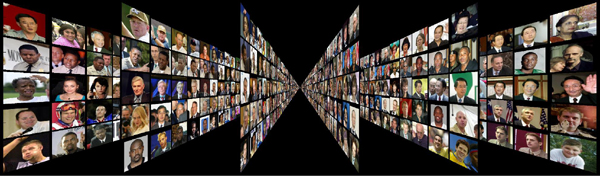
\includegraphics[scale=0.3]{lfw}
\caption{Labeled Faces in the Wild Dataset}
\label{fig:lfw}
\end{figure}
\section{Algorithms}

\subsection{OpenCV}
The start of facial recognition relies on detecting the faces to identify the landmark locations
and the bounding box for the face. The two foundational methods are looking at HAAR like
features and HOG. The OpenCV library uses a HAAR-like features and a cascaded classifier
structure \cite{Viola2001}. This means that the classifiers are applied to a region of
interest in the picture and if the classifier passes then another classifier which consists of the
previous simpler classifier is used to check the image. This cascading effect allows the parts of
the image to be refined through the cascading effect of the classifiers or to be rejected early
on by the simpler classifiers as not to waste processing power. The Haar-like features looks at
rectangular regions that are adjacent to each other, it adds up the pixel intensities in the
regions then looks at the difference between the sums. This value is then used to describe the
region of the image. The cascades are necessary as using only a simple Haar-like feature
classifier isn’t robust, to create a stronger classifier they must be cascaded and combined
together using an adaboost bosting technique to gain better accuracy \cite{Rahmad2020}.
The original Viola and Jones algorithm which uses Haar-like features for object detection can
be implemented through the use of OpenCV \cite{Naveenkumar2016}.
\begin{figure}[h!]
\centering
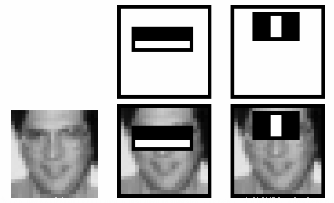
\includegraphics[scale=0.4]{haar}
\caption{Haar-like features}
\label{fig:haar}
\end{figure}
\subsection{DLIB}
DLIB takes a state of the art approach and uses a HOG feature descriptor with a linear
SVM machine learning algorithm \cite{Dalal2005}. It works by splitting the image into a
grid first and for every grid square it assigns it’s a histogram based on direction of gradients.
Next all the histograms are brought together to form one histogram which can uniquely
describe each face. This is used with a linear SVM classifier to provide face detection. More
recently CNN have started to be used as facial detection methods as the it provides better
accuracy for faces that are not full frontal facing.
\subsection{R-CNN}
Faster R-CNN \cite{Ren2017} is another method for object detection, it’s a family of
algorithms that span through speed and efficiency. It works by leveraging the idea of Region
Proposal Networks to reduce the number of candidates. Facial detection through CNN’s can
be very expensive in terms of computational power so it is in best interest that the amount of
work required be reduced by removing certain candidates. The original R-CNN algorithm
works by using a selective search algorithm to break down the images into smaller sections
and then bringing them together to create objects. This is based on the texture, colour, size
and shape, these become our region proposals which then form a feature length vector. A
SVM similar to that in DLIB is used to classify the objects and then to gain a more accurate
bounding box, regression is done. Fast R-CNN was built upon this by instead of generating
region proposals for the CNN, now the CNN is fed the image and a convolutional feature map
is generated from this. This map is then used to identify regions, it reduces the need to feed
in 2000 separate region proposals which greatly improves the performance. The Faster R-CNN
algorithm takes the previous and replaces the selective search with a network to predict region
proposals. This is extremely fast compared to the previous ones and can be used for real time
detection.
\subsection{MTCNN}
MTCNN \cite{Zhang2016} is another method proposed for facial detection it stands for
multitask cascaded neural network. It works using 3 networks; P-Net, R-Net and O-net. P-Net
is the proposal network and its job is to find the bounding box of faces based on estimations
of the bounding box. The next stage is the refinement network, which is where false candidates
are rejected, and calibration is performed. The final stage like the previous stage also performs
refinement but is called the output stage as it proposes the facial landmarks. The model learns
by back-propagating the error and changing the weights. The reason this algorithm is an
interesting one to look at, is that it doesn’t use a pre-existing face detection method and
instead uses its own shallow network and refinement to gather the information.
\begin{figure}[h!]
\centering
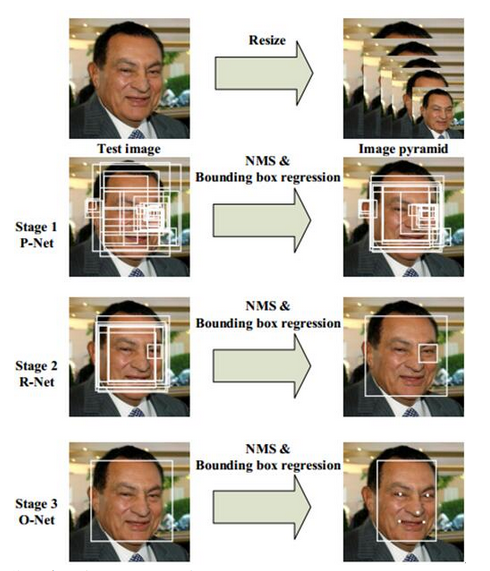
\includegraphics[scale=0.4]{mtcnn}
\caption{Neural Network Layers}
\label{fig:mtcnn}
\end{figure}

\subsection{Single Stage Detectors}
Single Stage Detectors are a class of algorithms that work through only one stage, i.e they
don’t use region proposals like the R-CNN algorithms. The YOLO v3 \cite{Redmon2016}
algorithm is a popular one, it stands for ‘You Only Look Once’. It works by using a single deep
neural network to predict where the bounding boxes are and the classification of them at the
same time. This algorithm is quick as it removes the need for identifying region proposals and
instead combines this and classification into the same step within the network.
Another single stage detection algorithm is Retina Face \cite{Deng2019} which can predict
the face score, face box and facial landmarks at the same time. Its based-on pixel-wise location
and feature pyramids to predict the face regions


\section{Feasibility}
The feasibility of this project is determined on many factors, these being availability,
computational power and ease of use.
In terms of availability I am referring to the availability of the facial detection algorithms. In
my case I would require open source algorithms as these would be free and ideally well
supported because they are so widely available. Fortunately, there are many libraries
available that provide an open source solution and implementation of many face detection
algorithms that I can use.
\newline \newline
Computation power is a concern to me during this project as my personal set up is a laptop
that may be able to run older algorithms like Viola and Jones but with only an integrated
graphics card I really lack computational power to run these CNN algorithms on multiple
image groups. If I have to train models, then this will wont be feasible as I don’t have the
power or time to achieve this. This being said I am able to use Google Collab to run the more
expensive algorithms, Google Collab is a cloud based python notebook which allows me to
connect to more powerful GPU’s to help tackle my machine learning and facial detection
tasks. I think this would be the sensible platform for me to run any code required for my 
project on as it greatly helps my computational power and reduces unnecessary setup
complexities on my local machine.
\newline \newline
Since I am not an expert in computer vision algorithms or CNN’s I would avoid choosing
algorithms that are too complicated for the project as I feel like I wouldn’t be able to draw
effective results from these. I do wish to find a middle ground between the cutting edge
algorithms and algorithms that are easier to use and implement as this would allow me to
more successfully analyse the sensitivity of the algorithm to race and gender. With my
selection of open source algorithms I feel like I have got a suitable range of algorithms that
represent the landscape of facial analysis and are still easy enough to implement

\section{Conclusion}
The different methods require different computational power to run and the differing data
sets might make it difficult to provide a comparison across models with the same dataset.
Working from home it might not be feasible to train a model myself with thousands of images,
but most algorithms come with pretrained models I could use. This means I wouldn’t entirely
be comparing algorithms but instead looking for a race and gender bias within the algorithms
which I think is more feasible.
Certain algorithms are more feasible to be used such as MTCNN, HOG, Viola and Jones and
Retina Face. These are accessible through open source technology and provide 3 techniques
in facial analysis that are varied enough to describe the industries conception to its current
state. I also think it would be fair to look at the different datasets each model is trained with
and compare these in terms of representation. 
\newpage
\bibliographystyle{plain}
\bibliography{references}
\end{document}
